\newpage
\def\thoigian{90}%--Thời gian
\de{Đề số 2}{Đề ôn tập Chương VIII - Quan hệ vuông góc}

\begin{center}
	\textbf{PHẦN 1 - Câu trắc nghiệm nhiều phương án lựa chọn.}
\end{center}
\setcounter{ex}{0}
\Opensolutionfile{ans}[ans-ABCD]

\begin{ex}%[1H8N1-3]
	Cho hình chóp $S.ABCD$ có đáy $ABCD$ là hình bình hành và tam giác $SAD$ vuông tại $A$. Góc giữa hai đường thẳng $SA$ và $BC$ là
	\choice
	{$30^\circ$}
	{$60^\circ$}
	{$45^\circ$}
	{\True $90^\circ$}
	\loigiai{
		\immini{Ta có $ AD\parallel BC\Rightarrow (SA,BC)=(SA,AD)=\widehat{SAD}=90^\circ $.}{\begin{tikzpicture}[scale=.7,font=\footnotesize, line join=round, line cap=round, >=stealth]
				\coordinate (A) at (0,0);
				\coordinate (D) at (5,0);
				\coordinate (B) at (-2,-2);
				\coordinate (C) at ($(B)+(D)-(A)$);
				\coordinate (S) at ($(A)+(0,4)$);
				\foreach \x/\g in {A/160,B/-100,C/-60,D/20,S/90} \fill[black](\x) circle (1.5pt) ($(\x)+(\g:3mm)$) node{$\x$};
				\draw (S)--(B)--(C)--(D)--(S)--(C);
				\draw[dashed] (B)--(A)--(D)
				(S)--(A);
		\end{tikzpicture}}	
	}
\end{ex}


\begin{ex}%[1H8N2-1]
	Qua điểm $O$ cho trước có bao nhiêu mặt phẳng vuông góc với đường thẳng $\Delta$ cho trước
	\choice
	{$2$}
	{Vô số}
	{$3$}
	{\True $1$}
	\loigiai{Có duy nhất một mặt phẳng đi qua điểm $ O $ cho trước và vuông góc với đường thẳng $\Delta$ cho trước.}
\end{ex}


\begin{ex}%[1H8H2-2]
	\immini[thm]{Cho hình chóp $S.ABCD$ có đáy $ABCD$ là hình bình hành tâm $O$; $SA=SC$; $SB=SD$ (tham khảo hình bên). Khẳng định nào sau đây là đúng?
		\choice
		{\True $SO\perp(ABCD)$}
		{$SB\perp(SCD)$}
		{$SA\perp(ABCD)$}
		{$SC\perp(SBD)$}}{\begin{tikzpicture}[scale=.7,font=\footnotesize, line join=round, line cap=round, >=stealth]
			\coordinate (A) at (0,0);
			\coordinate (D) at (5,0);
			\coordinate (B) at (-2,-2);
			\coordinate (C) at ($(B)+(D)-(A)$);
			\coordinate (O) at ($(C)!0.5!(A)$);
			\coordinate (S) at ($(O)+(0,5)$);
			\foreach \x/\g in {A/160,B/-100,C/-60,D/20,S/90,O/-90} \fill[black](\x) circle (1.5pt) ($(\x)+(\g:3mm)$) node{$\x$};
			\draw (S)--(B)--(C)--(D)--(S)--(C);
			\draw[dashed] (B)--(A)--(D)--(B)
			(O)--(S)--(A)--(C);
	\end{tikzpicture}}
	\loigiai{Tam giác $ SAC $ cân tại $ S $ có $ O $ là trung điểm của cạnh $ AC $ nên $ SO\perp AC $.\\
		Tam giác $ SBD $ cân tại $ S $ có $ O $ là trung điểm của cạnh $ BD $ nên $ SO\perp BD $.\\
		Suy ra $ SO\perp (ABCD) $. }
\end{ex}


\begin{ex}%[1H8H2-2]
	Cho hình lập phương $ABCD.A'B'C'D'$. Đường thẳng $AC'$ vuông góc với mặt phẳng nào sau đây?
	\choice
	{\True $(A'BD)$}
	{$(A'DC')$}
	{$(A'CD')$}
	{$(A'B'CD)$}
	\loigiai{\immini{
			Ta có $\heva{& BD\perp AC \\ & BD\perp AA'}$ nên $BD\perp ( ACC'A')$.\\
			Mà $AC'\subset ( ACC'A')$ nên $ AC'\perp BD $.\\
			Ta lại có $\heva{& A'B\perp AB' \\ & A'B\perp B'C'}$ nên $A'B\perp ( AB'C'D)$.\\
			Mà $AC'\subset ( AB'C'D)$ nên $ AC'\perp A'B $.\\
			Từ chứng minh trên suy ra $ AC' \perp (A'BD) $.
		}
		{\begin{tikzpicture}[scale=.7, font=\footnotesize, line join=round, line cap=round, >=stealth]
				\def\bc{4} % cạnh BC
				\def\ba{2} % cạnh BA
				\def\gocB{40} % góc B của đáy
				\coordinate[label=below left:$B$] (B) at (0,0);
				\coordinate[label=left:$A$] (A) at (\gocB:\ba);
				\coordinate[label=below:$C$] (C) at (\bc,0);
				\coordinate[label=right:$D$] (D) at ($(C)-(B)+(A)$);
				\coordinate[label=above left:$A'$] (A') at ($(A)+(90:\bc)$);
				\coordinate[label=left:$B'$] (B') at ($(B)-(A)+(A')$);
				\coordinate[label=below right:$C'$] (C') at ($(C)-(A)+(A')$);
				\coordinate[label=right:$D'$] (D') at ($(D)-(A)+(A')$);
				\draw (B')--(B)--(C)--(D)--(D')--(A')--(B')--(C')--(D') (C)--(C');
				\draw[dashed] (B)--(A')--(D)--(A)--(B') (C')--(A)--(B)--(D) (A')--(A)--(C) ;
				\foreach \diem in {A,B,C,D,A',B',C',D'}	\fill (\diem)circle(1.5pt);
			\end{tikzpicture}
	}}
\end{ex}

\begin{ex}%[1H8H6-1]
	Cho hình chóp $S.ABC$ có $SA\perp(ABC)$. Góc giữa đường thẳng $SC$ và mặt phẳng $(ABC)$ là
	\choice
	{$\widehat{SAC}$}
	{$\widehat{SBC}$}
	{\True$\widehat{SCA}$}
	{$\widehat{SCB}$}
	\loigiai{\immini{Vì $SA\perp(ABC)$ nên $AC$ là hình chiếu của $SC$ trên $(ABC)$.\\
			Suy ra $( SC,( ABC))=( SC,AC)=\widehat{SCA}$. }
		{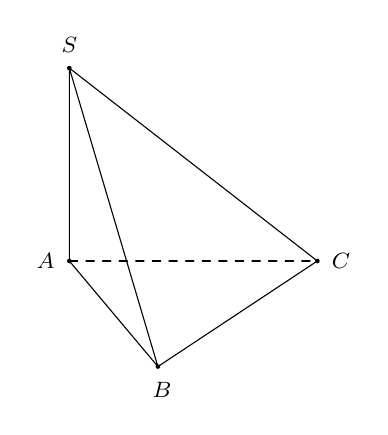
\begin{tikzpicture}[scale=0.7, font=\footnotesize, line join=round, line cap=round,>=stealth]
				\path (0,0) coordinate (A)
				+(-50:2.5) coordinate (B)
				+(0:4.5) coordinate (C)
				+(90:3.5) coordinate (S)
				;
				\draw (S)--(A)--(B)--(S)--(C)--(B);
				\draw[dashed] (A)--(C);	
				\foreach \p/\q in {A/180,C/0,B/-80,S/90}{
					\path (\p) node[shift={(\q:3mm)}]{$\p$};
					\fill[black] (\p) circle (1.2pt);}
	\end{tikzpicture}}}
\end{ex}


\begin{ex}%[1H8H6-2]
	\immini[thm]{
		Cho hình chóp $S.ABCD$ có đáy $ABCD$ là hình vuông cạnh $a$, $SA$ vuông góc với đáy và $SA=\dfrac{a\sqrt{6}}{6}$.	Số đo góc nhị diện $[S,BD,C]$ bằng
		\choice
		{$30^{\circ}$}
		{$45^{\circ}$}
		{$60^{\circ}$}
		{\True $150^{\circ}$}
	}{
		\begin{tikzpicture}[scale=1,>=stealth, font=\footnotesize, line join=round, line cap=round]
			\coordinate (A) at (0,0);
			\coordinate (B) at (-1.3,-1.6);
			\coordinate (D) at (3.5,0);
			\coordinate (C) at ($(B)+(D)-(A)$);
			\coordinate (S) at ($(A)+(0,2)$);
			\draw (S)--(B)--(C)--(D)--cycle
			(S)--(B) (S)--(C);
			\draw[dashed] (A)--(B)--(D) (A)--(D) (S)--(A);
			\foreach \p/\r in {S/90,A/180,B/-90,C/-45,D/0}
			\fill (\p) circle (1pt) node[shift={(\r:3mm)}]{$\p$};
		\end{tikzpicture}
	}
	\loigiai{
		\immini{
			$ABCD$ là hình vuông nên $AC\perp BD$ hay $OC\perp BD$.\\
			$\heva{&BD\perp AC\\&BD\perp SA} \Rightarrow BD\perp (SAC).$\\
			$\Rightarrow SO\perp BD$.\\
			Suy ra $\widehat{SOC}$ là góc phẳng nhị diện $[S,BD,C]$.\\
			Ta có $AC=AB\sqrt{2}=a\sqrt{2}\Rightarrow AO=\dfrac{a\sqrt{2}}{2}$.\\
			$\tan \widehat{SOA}=\dfrac{SA}{AO}=\dfrac{\dfrac{a\sqrt{6}}{6}}{\dfrac{a\sqrt{2}}{2}}=\dfrac{\sqrt{3}}{3}\Rightarrow \widehat{SOA}=30^\circ$.\\
			Suy ra $\widehat{SOC}=180^\circ-\widehat{SOA}=180^\circ-30^\circ=150^\circ$.\\
			Vậy số đo góc nhị diện $[S,BD,C]$ bằng $150^\circ$.
		}{
			\begin{tikzpicture}[scale=1,>=stealth, font=\footnotesize, line join=round, line cap=round]
				\coordinate (A) at (0,0);
				\coordinate (B) at (-1.3,-1.6);
				\coordinate (D) at (3.5,0);
				\coordinate (C) at ($(B)+(D)-(A)$);
				\coordinate (S) at ($(A)+(0,2)$);
				\path ($(A)!0.5!(C)$) coordinate (O);
				\draw (S)--(B)--(C)--(D)--cycle
				(S)--(B) (S)--(C);
				\draw[dashed] (A)--(B)--(D) (C)--(A)--(D) (O)--(S)--(A);
				\foreach \p/\r in {S/90,A/180,B/-90,C/-45,D/0,O/-80}
				\fill (\p) circle (1pt) node[shift={(\r:3mm)}]{$\p$};
				\draw pic[fill=yellow,draw=black,opacity=.5, angle eccentricity=1.2, angle radius=0.3cm]{angle=C--O--S};
			\end{tikzpicture}
		}
	}
\end{ex}

\begin{ex}%[1H8H1-3]
	Cho hình lập phương $ABC D.A' B' C' D'$. Góc giữa hai đường thẳng $BA'$ và $CD$ bằng
	\choice
	{\True $45^{\circ}$}
	{$60^{\circ}$}
	{$30^{\circ}$}
	{$90^{\circ}$}
	\loigiai{
		\immini{
			Ta có $BA' \parallel CD'$ nên $\left(BA',CD\right) = \left(CD',CD\right) = \widehat{DCD'}= 45^\circ $.
		}{
			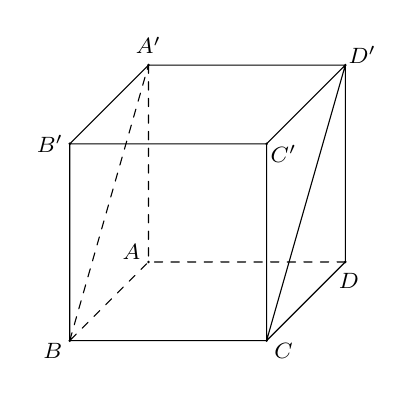
\begin{tikzpicture}[font=\footnotesize,line join=round, line cap=round, >=stealth,scale=0.5]
				\path
				(0,0) coordinate (A)
				(-2,-2) coordinate (B)	
				(3,-2) coordinate (C)	
				(5,0) coordinate (D)	
				(0,5) coordinate (A')	
				(-2,3) coordinate (B')	
				(3,3) coordinate (C')	
				(5,5) coordinate (D')	
				;
				\draw (B')--(B)--(C)--(C')--(B')--(A')--(D')--(C') (B)--(C)--(D)--(D') (C)--(D');
				\draw[dashed] (A')--(A)--(B) (D)--(A) (B)--(A');
				\foreach \x/\pos in{A/150,B/-150,C/-30,D/-80,A'/90,B'/180,C'/-30,D'/30}
				\fill (\x) circle(1pt) node[{shift=(\pos:0.25)}]{$\x$};
			\end{tikzpicture}
		}
	}
\end{ex}

\begin{ex}%[1H8H5-3]
	Cho hình chóp $S . A B C D$ có $S A \perp(A B C D)$ và đáy $A B C D$ là hình vuông cạnh $a$. Khoảng cách từ $C$ đến $(S A D)$ bằng
	\choice
	{$2a$}
	{\True $a$}
	{$a \sqrt{3}$}
	{$\dfrac{a}{2}$}
	\loigiai{
		\immini{
			Ta có $\heva{&CD\perp SA\\ &CD\perp AD}\Rightarrow CD\perp\left(SAD\right)$.\\
			Do đó $\mathrm{d}\big(C,(SAD)\big)=CD=a$.
		}{
			\begin{tikzpicture}[font=\footnotesize,line join=round, line cap=round, >=stealth,scale=0.6]
				\path
				(0,0) coordinate (A)
				(-2,-2) coordinate (B)	
				(3,-2) coordinate (C)	
				(5,0) coordinate (D)	
				(0,5) coordinate (S)	
				;
				\draw (S)--(B)--(C)--(S)--(D)--(C);
				\draw[dashed] (S)--(A)--(B) (A)--(D);
				\foreach \x/\pos in{A/150,B/-100,C/-80,D/-80,S/90}
				\fill (\x) circle(1pt) node[{shift=(\pos:0.25)}]{$\x$};
				\pic[draw,thin,angle radius=2mm] {right angle = S--A--D};
				\pic[draw,thin,angle radius=2mm] {right angle = B--A--D};
				\pic[draw,thin,angle radius=2mm] {right angle = A--D--C};
			\end{tikzpicture}
		}
	}
\end{ex}

\begin{ex}%[1H8N7-3]
	Cho hình chóp tứ giác $S.ABCD$ có đáy là hình vuông cạnh $a$, $SA$ vuông góc với mặt phẳng đáy và $SA=2a$. Thể tích khối chóp $S.ABCD$ bằng
	\choice
	{$2a^3$}
	{$\dfrac{a^3}{3}$}
	{\True $\dfrac{2a^3}{3}$}
	{$\dfrac{4a^3}{3}$}
	\loigiai{
		Ta có $V_{S.ABCD}=\dfrac{1}{3}\cdot SA\cdot S_{ABCD}=\dfrac{1}{3}\cdot 2a\cdot a^2=\dfrac{2a^3}{3}$.
	}
\end{ex}


\begin{ex}%[1H8H6-1]
	Hình chóp $S.ABC$ có $SA$ vuông góc với mặt đáy. Biết $SA=a$, $AC=a\sqrt{3}$. Khi đó góc giữa đường thẳng $SC$ và mặt phẳng $(ABC)$ có số đo là
	\choice
	{$90^\circ$}
	{$45^\circ$}
	{\True $30^\circ$}
	{$60^\circ$}
	\loigiai{
		Do $SA\perp (ABC)$ nên $\left(SC,(ABC) \right) =\widehat{SCA}$.\\
		Tam giác $SAC$ vuông tại $A$ nên $\tan \widehat{SCA} = \dfrac{SA}{AC}=\dfrac{a}{a\sqrt{3}}=\dfrac{1}{\sqrt{3}}\Rightarrow \widehat{SCA}=30^\circ$.
	}
\end{ex}
\begin{ex}%[1H8N7-6]
	Khối lăng trụ có chiều cao $h$ và diện tích đáy $B$ có thể tích là
	\choice
	{\True $Bh$}
	{$3Bh$}
	{$\dfrac{1}{3}Bh$}
	{$\dfrac{1}{2}Bh$}
	\loigiai
	{
		Khối lăng trụ có chiều cao $h$ và diện tích đáy $B$ có thể tích là $Bh$.
	}
\end{ex}

\begin{ex}%[1H8H7-3]
	Cho hình chóp $S.ABCD$ có đáy $ABCD$ là hình vuông cạnh bằng $a\sqrt{2}$, cạnh bên $SA$ vuông góc với đáy và $SA=a\sqrt{3}$. Thể tích khối chóp $S.ABCD$ bằng
	\choice
	{$\dfrac{a^3\sqrt{2}}{3}$}
	{\True $\dfrac{2a^3\sqrt{3}}{3}$}
	{$\dfrac{a^3\sqrt{3}}{3}$}
	{$2a^3\sqrt{3}$}
	\loigiai{
		\immini{
			Ta có $V = \dfrac{1}{3}\cdot \left( a\sqrt 2\right)^2 \cdot a\sqrt 3  = \dfrac{2a^3\sqrt{3}}{3}$
		}{
			\begin{tikzpicture}[font=\footnotesize,line join=round, line cap=round, >=stealth,scale=0.7]
				\path
				(0,0) coordinate (A)
				(-2,-2) coordinate (B)	
				(3,-2) coordinate (C)	
				(5,0) coordinate (D)	
				(0,5) coordinate (S)	
				;
				\draw (S)--(B)--(C)--(S)--(D)--(C);
				\draw[dashed] (S)--(A)--(B) (A)--(D);
				\foreach \x/\pos in{A/150,B/-100,C/-80,D/-80,S/90}
				\fill (\x) circle(1pt) node[{shift=(\pos:0.25)}]{$\x$};
				\pic[draw,thin,angle radius=2mm] {right angle = S--A--D};
				\pic[draw,thin,angle radius=2mm] {right angle = B--A--D};
				\pic[draw,thin,angle radius=2mm] {right angle = A--D--C};
			\end{tikzpicture}
		}
	}
\end{ex}
\Closesolutionfile{ans}

%\indapan{6}{ans-ABCD}

%\cauds

\begin{center}
	\textbf{PHẦN 2 - Câu trắc nghiệm đúng sai. Trong mỗi ý a,b,c,d ở mỗi câu, thí sinh chọn đúng hoặc sai}
\end{center}
\setcounter{ex}{0}
\Opensolutionfile{ans}[ans-DS]


\begin{ex}%[1H8H7-2]
	\immini[thm]{Cho hình chóp $S.ABCD$ có đáy $ABCD$ là hình vuông cạnh $a$. Mặt bên $SAB$ là tam giác đều và $SH\perp (ABCD)$ với $H$ là trung điểm của $AB$. Các mệnh đề sau đúng hay sai?
		\choiceTF
		{\True $SH\perp BD$}
		{$AB\perp (SAD)$}
		{\True $(SAB)\perp (SAD)$}
		{\True Thể tích khối chóp $S.ABC$ là $\dfrac{a^3\sqrt{3}}{12}$}
	}
	{\begin{tikzpicture}[>=stealth,line join=round,line cap=round,font=\footnotesize,scale=0.4]
			%\def\r{6.5};
			\clip (-5,-5) rectangle (10,7);
			\path
			(0,0) coordinate (A)
			(-4,-4) coordinate (B)
			(5,-4) coordinate (C)
			(9,0) coordinate (D)
			(-2,-2) coordinate (H)
			(-2,6) coordinate (S)
			;
			\draw  (S)--(B)--(C)--(D)--(S)--(C);
			\draw[dashed](B)--(A)--(D)(A)--(S)--(H)(A)--(C)(B)--(D);
			%\path[name path=d1] (A)--(C) ;% Gán tên đường $AC$ là $d1$.
			\fill[black] (A) circle (1.5pt) node[above left]{$A$}(C) circle (1.5pt) node[below right]{$C$}(B) circle (1.5pt) node[below left]{$B$}(S) circle (1.5pt) node[above]{$S$}(H) circle (1.5pt) node[below right]{$H$}(D) circle (1.5pt) node[below right]{$D$};
			%\draw (O) circle (\r);
			%($(A)!(B)!(C)$) coordinate (F)
			%\path[name path=c1] (I) let \p1=($(I)-(B)$) in circle({veclen(\x1,\y1)});
			\draw pic[draw, opacity = .7, angle radius = 5pt] {right angle =S--H--A};%Vẽ góc vuông BKC
	\end{tikzpicture}}
	\loigiai{
		\begin{itemize}
			\item Vì $SH\perp (ABCD)$ nên $SH\perp BD$.
			\item Do $\triangle SAB$ đều nên $AB \not \perp SA\Rightarrow AB \not \perp (SAD)$.
			\item Ta có $\heva{&AD\perp AB\\&AD\perp SH}\Rightarrow AD\perp (SAB)\Rightarrow (SAD)\perp (SAB)$.
			\item Ta có $V_{S.ABC}=\dfrac{1}{3}\cdot SH\cdot S_{ABC}$.
			Tam giác $SAB$ đều cạnh $a$ nên $SH=\dfrac{a\sqrt{3}}{2}$. Lại có $S_{ABC}=\dfrac{a^2}{2}$. Do đó
			\[V_{S.ABC}=\dfrac{1}{3}\cdot \dfrac{a\sqrt{3}}{2}\cdot \dfrac{a^2}{2} =\dfrac{a^3\sqrt{3}}{12}.\]
		\end{itemize}
	}	
\end{ex}

\begin{ex}%[1H8H6-1]
	\immini[thm]{
		Cho hình chóp $S.ABCD$ có đáy $ABCD$ là hình vuông cạnh $a$, $SA$ vuông góc với mặt phẳng đáy và $SA=a$. Xác định khẳng định đúng trong các khẳng định dưới đây.
		\choiceTF
		{\True $SA\perp BC$}
		{$SD\perp (ABCD)$}
		{\True Góc giữa đường thẳng $SC$ và mặt phẳng $(ABCD)$ là $\widehat{SCA}$}
		{Khoảng cách từ điểm $A$ đến mặt phẳng $(SBC)$ là $a\sqrt{2}$}
	}{
		\begin{tikzpicture}[scale=0.8, line join=round, line cap=round, >=stealth]
			\coordinate (A) at (0,0);
			\coordinate (D) at (3,0);
			\coordinate (B) at (-2,-1);
			\coordinate (C) at ($(D)-(A)+(B)$);
			\coordinate (x) at (0,3);
			\coordinate (S) at ($(A)+(x)$);
			\draw (S)--(B)--(C)--(D)--(S)--(C);
			\draw[dashed] (S)--(A)--(D)
			(A)--(B);
			\foreach \x/\g in {A/150,B/-90,C/-90,D/30,S/90} \fill[black](\x) circle (1pt)+(\g:0.3)node{$\x$};
		\end{tikzpicture}
	}
	\loigiai{
		\begin{center}
			\begin{tikzpicture}[scale=0.8, line join=round, line cap=round, >=stealth]
				\coordinate (A) at (0,0);
				\coordinate (D) at (3,0);
				\coordinate (B) at (-2,-1);
				\coordinate (C) at ($(D)-(A)+(B)$);
				\coordinate (x) at (0,3);
				\coordinate (S) at ($(A)+(x)$);
				\coordinate (H) at ($(S)!0.5!(B)$);
				\draw (S)--(B)--(C)--(D)--(S)--(C);
				\draw[dashed] (S)--(A)--(D)
				(C)--(A)--(B)
				(H)--(A);
				\foreach \x/\g in {A/45,B/-90,C/-90,D/45,S/90,H/150} \fill[black](\x) circle (1pt)+(\g:0.3)node{$\x$};
			\end{tikzpicture}
		\end{center}
		\begin{itemchoice}
			\itemch Vì $SA\perp (ABCD)$ nên $SA\perp BC$.
			\itemch Ta có $SA\perp (ABCD)$. Nếu $SD\perp (ABCD)$ thì $S,A,D$ thẳng hàng, vô lí.
			\itemch Hình chiếu của $SC$ lên $(ABCD)$ là $AC$ nên góc giữa đường thẳng $SC$ và mặt phẳng $(ABCD)$ là $\widehat{SCA}$.
			\itemch Gọi $H$ là hình chiếu của $A$ lên $SB$.\\
			Ta có $\heva{& AH\perp SB \\ & AH \perp BC \quad (\text{do } BC\perp(SAB))}$ nên suy ra $AH\perp (SBC)$.\\
			Do đó khoảng cách từ điểm $A$ đến mặt phẳng $(SBC)$ là $AH$.\\
			Ta có $\dfrac{1}{AH^2}=\dfrac{1}{AS^2}+\dfrac{1}{AB^2}=\dfrac{1}{a^2}+\dfrac{1}{a^2}=\dfrac{2}{a^2}$. Suy ra $AH=\dfrac{a\sqrt{2}}{2}$.
		\end{itemchoice}
	}	
\end{ex}


\Closesolutionfile{ans}


\begin{center}
	\textbf{PHẦN 3 - Câu trắc nghiệm trả lời ngắn}
\end{center}
\setcounter{ex}{0}

\Opensolutionfile{ans}[ans-KQ]


\begin{ex}%[1H8H6-1]
	Cho hình chóp $S.ABCD$ có $SA\perp (ABCD)$, $ABCD$ là hình thang vuông tại $A$ và $D$, $AD=CD=a$, $AB=2a$, $SA=a\sqrt{2}$. Xác định góc giữa đường thẳng $SC$ và mặt phẳng $(SAD)$ theo đơn vị độ.
	\shortans[]{$30$}
	\loigiai{
		\immini{Ta có $\heva{&CD\perp AD\\&CD\perp SA}\Rightarrow CD\perp (SAD)$. Suy ra hình chiếu của $SC$ lên $(SAD)$ là $SD$. Do đó $\left(SC,(SAD)\right)=\left(SC,SD\right)=\widehat{CSD}$.\\
			Tam giác $CSD$ vuông tại $D$, ta có\\
			$\tan \widehat{CSD}=\dfrac{CD}{SD}=\dfrac{CD}{\sqrt{SA^2+AD^2}}=\dfrac{a}{a\sqrt{3}}=\dfrac{\sqrt{3}}{3}$\\
			$\Rightarrow \widehat{CSD}=30^{\circ}$.
		}
		{\begin{tikzpicture}[>=stealth,line join=round,line cap=round,font=\footnotesize,scale=0.4]
				%\def\r{6.5};
				\clip (-5,-5) rectangle (13,9);
				\path
				(0,0) coordinate (A)
				(-4,-4) coordinate (D)
				(2,-4) coordinate (C)
				(12,0) coordinate (B)
				(0,8) coordinate (S)
				;
				\draw  (S)--(B)--(C)--(D)--(S)--(C);
				\draw[dashed](B)--(A)--(D)(A)--(S);
				%\path[name path=d1] (A)--(C) ;% Gán tên đường $AC$ là $d1$.
				\fill[black] (A) circle (1.5pt) node[above left]{$A$}(C) circle (1.5pt) node[below right]{$C$}(B) circle (1.5pt) node[below right]{$B$}(S) circle (1.5pt) node[above]{$S$}(D) circle (1.5pt) node[below right]{$D$};
				\draw  (5,0)node[above left]{$2a$}(-2,-2)node[above left]{$a$}(-2,-4)node[below]{$a$}(0,2)node[left]{$a\sqrt{2}$};
				%\draw (O) circle (\r);
				%($(A)!(B)!(C)$) coordinate (F)
				%\path[name path=c1] (I) let \p1=($(I)-(B)$) in circle({veclen(\x1,\y1)});
				\draw pic[draw, opacity = .7, angle radius = 5pt] {right angle =S--A--B};%Vẽ góc vuông BKC
				\draw pic[draw, opacity = .7, angle radius = 5pt] {right angle =S--A--D};
				\draw pic[draw, opacity = .7, angle radius = 5pt] {right angle =C--D--A};
				\draw pic[draw, opacity = .7, angle radius = 5pt] {right angle =D--A--B};
				\draw pic[draw, fill = gray!50,opacity = .7, angle radius = 15pt] {angle =D--S--C};
		\end{tikzpicture}}
	}
\end{ex}


\begin{ex}%[1H8C5-4]
	Cho hình chóp $S.ABCD$ có $SA\perp (ABCD)$, $ABCD$ là hình thang vuông tại $A$ và $D$, $AD=CD=a$, $AB=2a$, $SA=a\sqrt{2}$. Gọi $E$ là trung điểm của $BC$. Tính khoảng cách giữa hai đường thẳng $AE$ và $SB$ với $a=\sqrt{3}$.
	\shortans[]{$1$}
	\loigiai{
		\immini{Từ $B$ kẻ đường thẳng song song với $AE$, cắt $AD$ tại $F$.\\
			Kẻ $AK\perp BF$ tại $K$. Lại có $BF\perp SA$ nên $BF\perp (SAK)$. Suy ra $(SBF)\perp (SAK)$.\\
			Kẻ $AH\perp SK$ tại $H$, suy ra $AH\perp (SBF)$.\\
			Ta có $AE\parallel BF\Rightarrow AE\parallel (SBF)$, do đó
			\[\mathrm{d}\left(AE,SB\right)=\mathrm{d}\left(AE,(SBF)\right)=\mathrm{d}\left(A,(SBF)\right)=AH.\]
			Tam giác $SAK$ vuông tại $A$ có $AH$ là đường cao nên
			\[AH=\dfrac{SA\cdot AK}{\sqrt{SA^2+AK^2}}.\quad (1)\]
		}
		{\begin{tikzpicture}[>=stealth,line join=round,line cap=round,font=\footnotesize,scale=0.4]
				%\def\r{6.5};
				\clip (-5,-5) rectangle (13,9);
				\path
				(0,0) coordinate (A)
				(-4,-4) coordinate (D)
				(2,-4) coordinate (C)
				(12,0) coordinate (B)
				(0,8) coordinate (S)
				(7,-2) coordinate (E)
				(6,0) coordinate (M)
				(9,0) coordinate (N)
				;
				\coordinate (X) at ($(A)-(E)+(B)$);
				\coordinate (Y) at ($(B)!1.5!(X)$);
				\coordinate (Z) at ($(D)!2!(A)$);
				\path[name path=d1] (B)--(Y);
				\path[name path=d2] (Z)--(A) ;
				\path[name intersections={of=d1 and d2}] (intersection-1) coordinate (F);
				\coordinate (K) at ($(F)!0.25!(B)$);
				\coordinate (H) at ($(S)!(A)!(K)$);
				\draw  (S)--(B)--(C)--(D)--(S)--(C);
				\draw[dashed](B)--(A)--(D)(A)--(S)(A)--(E)(B)--(F)--(A)(S)--(F)(A)--(K)--(S)(A)--(H)(C)--(M)(E)--(N);
				%\path[name path=d1] (A)--(C) ;% Gán tên đường $AC$ là $d1$.
				\fill[black] (A) circle (1.5pt) node[above left]{$A$}(C) circle (1.5pt) node[below right]{$C$}(B) circle (1.5pt) node[below right]{$B$}(S) circle (1.5pt) node[above]{$S$}(D) circle (1.5pt) node[below right]{$D$}(E) circle (1.5pt) node[below right]{$E$}(F) circle (1.5pt) node[left]{$F$}(K) circle (1.5pt) node[above right]{$K$}(H) circle (1.5pt) node[right]{$H$}(M) circle (1.5pt) node[above right]{$M$}(N) circle (1.5pt) node[above right]{$N$};
				\draw  (5,0)node[above left]{$2a$}(-2,-2)node[above left]{$a$}(-2,-4)node[below]{$a$}(0,2)node[left]{$a\sqrt{2}$};
				%\draw (O) circle (\r);
				%($(A)!(B)!(C)$) coordinate (F)
				%\path[name path=c1] (I) let \p1=($(I)-(B)$) in circle({veclen(\x1,\y1)});
				\draw pic[draw, opacity = .7, angle radius = 5pt] {right angle =S--A--B};%Vẽ góc vuông BKC
				\draw pic[draw, opacity = .7, angle radius = 5pt] {right angle =S--A--D};
				\draw pic[draw, opacity = .7, angle radius = 5pt] {right angle =C--D--A};
				\draw pic[draw, opacity = .7, angle radius = 5pt] {right angle =D--A--B};
				\draw pic[draw, opacity = .7, angle radius = 5pt] {right angle =A--K--B};
				\draw pic[draw, opacity = .7, angle radius = 5pt] {right angle =A--H--K};
				\draw pic[draw, fill = gray!50, opacity = .7, angle radius = 20pt] {angle =F--B--A};
				\draw pic[draw, fill = gray!50, opacity = .7, angle radius = 20pt] {angle =E--A--N};
				\draw pic[draw, opacity = .7, angle radius = 5pt] {right angle =C--M--A};
				\draw pic[draw, opacity = .7, angle radius = 5pt] {right angle =E--N--A};
		\end{tikzpicture}}
		\noindent
		Lấy $M$, $N$ lần lượt là trung điểm của $AB$ và $BM$. Khi đó $ADCM$ là hình vuông cạnh $a$, $AN=\dfrac{3a}{2}$. \\
		Lại có $EN$ là đường trung bình của tam giác $BCM$ nên $EN=\dfrac{a}{2}$.\\
		Hai tam giác vuông $ANE$ và $BAF$ có $\widehat{NAE}=\widehat{ABF}$ nên đồng dạng. Do đó
		\[\dfrac{AF}{NE}=\dfrac{AB}{NA}\Rightarrow AF=\dfrac{AB\cdot NE}{NA}=\dfrac{2a\cdot \dfrac{a}{2}}{\dfrac{3a}{2}}=\dfrac{2a}{3}.\]
		Tam giác $ABF$ vuông tại $A$ có $AK$ là đường cao nên
		\[AK=\dfrac{AB\cdot AF}{\sqrt{AB^2+AF^2}}=\dfrac{2a\cdot \dfrac{2a}{3}}{\sqrt{4a^2+\dfrac{4a^2}{9}}}=\dfrac{a\sqrt{10}}{5}.\]
		Thay vào $(1)$ ta được
		\[AH=\dfrac{a\sqrt{2}\cdot \dfrac{a\sqrt{10}}{5}}{\sqrt{2a^2+\dfrac{2a^2}{5}}}=\dfrac{a\sqrt{3}}{3}=\dfrac{\sqrt{3}\cdot \sqrt{3}}{3}=1.\]
	}
\end{ex}
\begin{ex}%[1H8V5-4]
	Cho hình chóp $S .ABCD$ có đáy $ABCD$ là hình vuông cạnh $\sqrt{6}$, cạnh bên $SD=2 \sqrt{3}$ và $SD$ vuông góc với mặt phẳng đáy. Khoảng cách giữa hai đường thẳng $SB$ và $CD$ bằng
	\shortans[]{$2$}
	\loigiai{
		\immini{Ta có $\heva{&AB \perp SD \\& AB \perp AD \\& SD \cap AD=D \text { trong }(SAD)} \Rightarrow AB \perp(SAD)$.\\
			Vẽ $DH \perp SA$ tại $H$ trong mặt phẳng $(SAD)$.\\
			Ta có $\heva{&DH \perp AB \\& DH \perp SA} \Rightarrow DH \perp(SAB)$.
		}
		{	\begin{tikzpicture}[>=stealth,line join=round,line cap=round,font=\footnotesize,scale=0.8]
				\def\r{3}
				\path
				(0,0) coordinate (D)
				(-1.5,-2) coordinate (A)
				(5,0) coordinate (C)
				($(A)+(C)-(D)$) coordinate (B)
				($(D)+(0,4)$) coordinate (S)
				($(S)!0.45!(A)$) coordinate (H)
				;
				\draw (S)--(A)--(B)--(S)--(C)--(B);
				\draw[dashed] (H)--(D)--(C)(S)--(D)--(A);
				\foreach \x/\y in {D/-80,H/180,A/180,B/-90,C/16,S/90}
				\draw[fill=black] (\x) circle (1.1pt) + (\y:0.3cm) node{$\x$};
			\end{tikzpicture}
		}
		\noindent
		Vì $C D\parallel (S A B)$ nên $\mathrm{d}(S B ; C D)=\mathrm{d}((S A B) ; C D)=\mathrm{d}((S A B) ; D)=D H$.\\
		$\triangle S A D$ vuông tại $D$ với đường cao $D H$ có $D H=\dfrac{S D \cdot D A}{\sqrt{S D^2+D A^2}}=\dfrac{2 \sqrt{3} \cdot \sqrt{6}}{\sqrt{(2 \sqrt{3})^2+(\sqrt{6})^2}}=2$.
	}
	
\end{ex}

\begin{ex}%[1H8H6-1]
	Cho lăng trụ $ABC.A'B'C'$ có đáy là tam giác đều cạnh $a$, cạnh bên $BB'$ vuông góc với đáy, $BB'=2a$. Gọi $M$ là trung điểm của $BC$, gọi $\phi$ là góc giữa đường thẳng $A'M$ và mặt phẳng $(A'B'C')$. Tính $\tan \phi$ (làm tròn đến hàng phần trăm).
	\shortans[]{$2{,}31$}
	\loigiai
	{\immini{Gọi $H$ là trung điểm $B'C'$, ta có $MH\perp (A'B'C')$\\
			$\Rightarrow A'H$ là hình chiếu vuông góc của $A'M$ lên $(A'B'C')$.\\
			Suy ra góc giữa $A'M$ và $(A'B'C')$ là $\widehat{MA'H}$.\\
			Xét $\triangle A'HM$ vuông tại $H$, có $\tan\widehat{MA'H}=\dfrac{MH}{A'H}=2a\cdot\dfrac{2}{a\sqrt{3}}=\dfrac{4}{\sqrt{3}}$.\\ Vậy $\tan \phi\approx 2{,}31$.}{\begin{tikzpicture}[scale=0.8,font=\footnotesize,line join = round, line cap = round, >= stealth]
				\coordinate (A) at (0,0);
				\def\x{4}
				\def\y{2}
				\def\z{3}
				\def\g{-40}% goc  đáy
				\def\n{90} %goc nghiêng
				\coordinate (B) at ($(A)+(\x,0)$);
				\coordinate (C) at ($(A)+(\g:\y)$);
				\coordinate (A') at ($(A)+(\n:\z)$);
				\coordinate (B') at ($(B)+(\n:\z)$);
				\coordinate (C') at ($(C)+(\n:\z)$);
				\coordinate (M) at ($(C)!.5!(B)$);
				\coordinate (H) at ($(B')!.5!(C')$);
				\draw (A)--(C)--(C')--(A')--cycle;
				\draw (A')--(B')--(C')
				(B')--(B)--(C)--(C')
				(A')--(H)--(M)
				;
				\draw[dashed] (A)--(B)
				(A')--(M)
				;
				\begin{scope}
					\clip (M)--(A')--(H);
					\draw (A') circle (10pt);
				\end{scope}
				\foreach \p/\g in {A/-120,B/-90,C/-45,A'/180,B'/90,C'/70,H/-20,M/-20} \draw[blue,fill=white] (\p) circle(.5pt) node [shift={(\g:.3)}] {$\p$};
		\end{tikzpicture}}
	}
\end{ex}

\Closesolutionfile{ans}
\begin{center}
	\textbf{PHẦN 4 - Phần tự luận}
\end{center}
\setcounter{ex}{0}

\Opensolutionfile{ans}[ans-TL]


\begin{ex}%[1H8V5-4]
	Cho hình chóp $S.ABCD$ có đáy $ABCD$ là hình vuông cạnh $2a$, $O$ là giao điểm của $AC$ và $BD$, $SB=a\sqrt{7}$ và $SB$ vuông góc với mặt phẳng đáy $ABCD$.
	\begin{enumerate}
		\item Chứng minh tam giác $SAD$ là tam giác vuông.
		\item Chứng minh $AC$ vuông góc với mặt phẳng $(SBD)$.
		\item Tính khoảng cách giữa hai đường thẳng $SO$ và $CD$.
	\end{enumerate}
	\loigiai
	{\begin{center}
			\begin{tikzpicture}[scale=1, font=\footnotesize,line join=round, line cap=round, >=stealth]
				\def\h{3}
				\path (0,0) coordinate (B)
				(-1.6,-1.4) coordinate (A)
				++(4,0) coordinate (D)
				($(B)+(D)-(A)$) coordinate(C)
				(0,\h) coordinate(S)
				($(A)!1/2!(C)$) coordinate(O)
				($(B)!1/2!(C)$) coordinate(M)
				($(S)!0.65!(M)$) coordinate(H);
				\draw (S)--(A)--(D)--(C)--(S)--(D);
				\draw[dashed] (S)--(B)--(A)--(C)--(B)--(D)
				(S)--(O)--(M)--(S) (B)--(H);
				\foreach \diem/\pos in {A/-90, D/-90, C/0, B/170, S/90, O/-90, M/45, H/50} \fill (\diem) node[shift={(\pos:0.3)}] {$\diem$} circle(1pt);
				\path pic[draw=red,angle radius=0.2cm, angle eccentricity=0.6]{right angle=S--B--A}
				pic[draw=red,angle radius=0.2cm, angle eccentricity=0.6]{right angle=S--B--C}
				pic[draw=red,angle radius=0.2cm, angle eccentricity=0.6]{right angle=B--A--D}
				pic[draw=red,angle radius=0.2cm, angle eccentricity=0.6]{right angle=A--O--D}
				pic[draw=red,angle radius=0.2cm, angle eccentricity=0.6]{right angle=B--M--O}
				pic[draw=red,angle radius=0.2cm, angle eccentricity=0.6]{right angle=B--H--M};
			\end{tikzpicture}
		\end{center}
		\begin{enumerate}
			\item Ta có $AD\perp SB$ (vì $SB\perp (ABCD)$), $AD\perp AB$ (vì $ABCD$ là hình vuông). Mà $AB$, $SB$ cùng nằm trong mặt phẳng $(SAB)$ và cắt nhau tại $B$, suy ra $AD\perp (SAB) \Rightarrow AD\perp SA$.\\
			Vậy tam giác $SAD$ vuông tại $A$.
			\item Ta có $AC\perp SB$ (vì $SB\perp (ABCD)$), $AC\perp BD$ (vì $ABCD$ là hình vuông). Mà $BD$, $SB$ cùng nằm trong mặt phẳng $(SBD)$ và cắt nhau tại $B$, suy ra $AC\perp (SBD)$.
			\item Gọi $M$ là trung điểm của $BC$, $H$ là chân đường vuông góc kẻ từ $B$ đến $SM$. Khi đó ta có:
			\begin{itemize}
				\item $OM$ là đường trung bình của tam giác $BCD$ nên $OM\parallel CD \Rightarrow CD\parallel (SOM)$.
				\item $OM\perp BC$, $OM\perp SB$ nên $OM\perp (SBC)$, suy ra $OM\perp BH$. Mà $BH\perp SM$, $SM$ cắt $OM$ tại $M$ và cùng nằm trong mặt phẳng $(SOM)$ nên $BH\perp (SOM)$.
				\item Vì $M$ là trung điểm của $BC$ và là giao điểm của $BC$ với $(SOM)$, $BH\perp (SOM)$ nên $$\mathrm{d}(CD,SO) = \mathrm{d}(C,(SOM)) = \mathrm{d}(B,(SOM)) = BH.$$
				Xét tam giác $SBM$ vuông tại $B$, có đường cao là $BH$. Do đó
				$$\dfrac{1}{BH^2}= \dfrac{1}{BM^2}+\dfrac{1}{SB^2} = \dfrac{1}{a^2} + \dfrac{1}{7a^2} = \dfrac{8}{7a^2} \Rightarrow BH=\dfrac{a\sqrt{14}}{4}.$$
			\end{itemize}
			Vậy khoảng cách giữa hai đường thẳng $SO$ và $CD$ là $\mathrm{d}(SO,CD)=\dfrac{a\sqrt{14}}{4}$.
	\end{enumerate}}
\end{ex}

\begin{ex}%[1H8V5-3]
	Cho hình chóp $S.ABC$ có đáy $ABC$ là tam giác cân tại $B$, $SA\perp(ABC)$, $AB=a$, $\widehat{ABC}=120^\circ$, $SA=\dfrac{3a}{2}$. Gọi $I$ là trung điểm của $AC$.
	\begin{enumerate}
		\item Chứng minh rằng $BI\perp(SAC)$.
		\item Tính thể tích khối chóp $S. ABC$.
		\item Tính góc giữa hai mặt phẳng $(SBI)$ và $(ABC)$.
		\end{enumerate}
	\loigiai{
		\begin{center}
			\begin{tikzpicture}[line join = round, line cap = round,>=stealth,font=\footnotesize,scale=1]
				\foreach \x/\y/\diem in {0/0/A,-1/-1.5/B,4/0/K,0/3.5/S} \coordinate (\diem) at (\x,\y);
				\coordinate (C) at ($(K)!3/2!($(B)+(K)-(A)$)$);
				\coordinate (I) at ($(A)!0.5!(C)$);
				\coordinate (H) at ($(S)!3/4!(K)$);
				\coordinate (L) at ($(S)!3/4!(C)$);
				\draw (S)--(B)--(C)--(K)--(S)--(C) (H)--(L);
				\draw[dashed] (B)--(A)--(K) (S)--(A)--(C) (H)--(A)--(L) (B)--(I)--(S);
				\def \dolongoc{5}
				\foreach \x/\dinh/\y in {S/A/B,S/A/K,B/I/A,A/H/S,K/H/L,A/K/C} \draw ($(\dinh)!\dolongoc pt!(\x)$)--($(\dinh)!\dolongoc pt!(\x)+(\dinh)!\dolongoc pt!(\y)-(\dinh)$)--($(\dinh)!\dolongoc pt!(\y)$);
				\foreach \diem/\goc in {A/180,B/180,C/-90,K/0,S/90,I/0,L/0,H/0} \fill[black](\diem) circle (1pt) ($(\diem)+(\goc:3mm)$) node{$\diem$};
			\end{tikzpicture}
		\end{center}
		\begin{enumerate}
			\item Vì tam giác $ABC$ cân tại $B$ có $I$ là trung điểm của $AC$ nên $BI \perp AC$.\\
			Vì $SA \perp (ABC)$ nên $SA \perp BI$.\\
			Ta có $\heva{&BI\perp AC\\&SA \perp BI\\& SA, AC \subset (SAC)\\&SA \cap AC=A}\Rightarrow BI \perp (SAC)$.
			\item $S_{ABC}=\dfrac{1}{2}\cdot AB\cdot BC \cdot \sin \widehat{ABC}=\dfrac{1}{2}\cdot a\cdot a \cdot \sin 120^{\circ}=\dfrac{a^2\sqrt{3}}{4}$.\\
			$V_{S.ABC}=\dfrac{1}{3}\cdot S_{ABC}\cdot SA=\dfrac{1}{3}\cdot \dfrac{a^2\sqrt{3}}{4}\cdot \dfrac{3a}{2}=\dfrac{a^3\sqrt{3}}{8}$.
			\item Ta có
			$\heva{&(SBC)\cap (ABC)=BI\\&BI \perp (SAC)\\&(SAC)\cap (SBI)=SI\\&(SAC)\cap (ABC)=AC}\Rightarrow \left((SBI),(ABC)\right)=(SI,AC)=\widehat{SIA}$.\\
			Vì tam giác $ABC$ cân tại $B$ nên $AI=AB\cdot \sin\widehat{ABI}=a\cdot \sin 60^{\circ}=\dfrac{a\sqrt{3}}{2}.\\
			\tan \widehat{SIA}=\dfrac{SA}{AI}=\dfrac{\dfrac{3a}{2}}{\dfrac{a\sqrt{3}}{2}}=\sqrt{3} \Rightarrow \widehat{SIA}=60^{\circ}$.\\
			Vậy $\left((SBI), (ABC)\right)=60^{\circ}$.
				\end{enumerate}
	}
\end{ex}


\begin{ex}%[1H8V6-7]
	Một nhóm sinh viên muốn dựng một chiếc lều trại hình chóp $S.ABC$ cho chuyến dã ngoại.
	\begin{itemize}
		\item Phần nền lều là tam giác $ABC$ được thiết kế là một tam giác đều với mỗi cạnh dài $3$ mét.
		\item Phần khung lều phía trước $SAB$ cũng được thiết kế là một tam giác đều với mỗi cạnh dài $3$ mét.
		\item Mặt phẳng chứa khung lều phía trước $(SAB)$ được dựng vuông góc với mặt phẳng nền lều $(ABC)$ để đảm bảo sự vững chắc.
	\end{itemize}
	Để kiểm tra độ dốc và ổn định của các mặt bên, nhóm cần tính toán góc nghiêng của mặt bên $(SBC)$ so với mặt phẳng nền lều $(ABC)$. Gọi $\alpha$ là góc phẳng nhị diện $[S,BC,A]$. Hãy giúp nhóm sinh viên tính giá trị của $\cos \alpha$ (làm tròn đến hàng phần trăm) để họ có thể điều chỉnh thiết kế nếu cần.
	\loigiai{
		\immini{
			Gọi $H$ là trung điểm của $AB$.\\
			Ta có $\triangle SAB$ là tam giác đều nên $SH\perp AB$.\\
			Lại có $(SAB)\perp (ABC)$, do đó $SH\perp (ABC)$.\\
			Gọi $M$ là hình chiếu của $H$ trên $BC$, khi đó
			\[\heva{&HM\perp BC\\&SH\perp BC\,\,(SH\perp (ABC)\supset BC)}\Rightarrow BC\perp (SHM)\Rightarrow BC\perp SM.\]
		}{
			\begin{tikzpicture}[>=stealth,line join=round,line cap=round,font=\footnotesize,scale=1.1]
				\tikzset{
					pics/chopTamGiac/.style n args={5}{
						code={
							\tikzset{declare function={a=3;b=2;h=3;goc=-130;}}
							\path
							(0,0)coordinate (#1)+(0:a)coordinate (#3)+
							(goc:b)coordinate (#2) ($(#1)!.5!(#2)$)coordinate (#4)
							($(#4)+(90:h)$)coordinate (#5)
							
							;
							\foreach \pointo/\pointt in {#2/#3,#3/#5,#5/#2}{
								\draw[fill=black](\pointo)--(\pointt);
							}
							\foreach \pointo/\pointt in {#1/#3,#1/#2,#1/#5,#5/#4}{
								\draw[fill=black,dashed](\pointo)--(\pointt);
							}
							
						}
				}}
				\path
				(0,0)coordinate (a)pic{chopTamGiac={A}{B}{C}{H}{S}}
				($(B)!.25!(C)$)coordinate (M)
				;
				\foreach \pointo/\pointt in {H/M}{
					\draw[fill=black,dashed](\pointo)--(\pointt);
				}
				\foreach \pointo/\pointt in {S/M}{
					\draw[fill=black](\pointo)--(\pointt);
				}
				\foreach \point/\goc in {S/90,A/50,B/-90,C/-10,H/10,M/-60}{
					\draw[fill=black](\point)circle(.8pt)+(\goc:2mm)node[scale=.8]{$\point$};
				}
			\end{tikzpicture}
		}
		Do đó $[S,BC,A]=\widehat{SMH}$.\\
		Ta có $\triangle SBC$ đều cạnh $3$, $SH$ là đường trung tuyến, do đó $SH=\dfrac{3\sqrt{3}}{2}$.\\
		Lại có $\triangle BHM$ vuông tại $M$, do đó \[HM=BH\cdot \sin B=\dfrac{3}{2}\cdot \sin 60^{\circ}=\dfrac{3\sqrt{3}}{4}.\]	
		Tam giác $SHM$ vuông tại $H$ nên $SM=\sqrt{SH^2+HM^2}=\dfrac{3\sqrt{15}}{4}$.\\
		Suy ra $\cos \alpha=\cos \widehat{SMH}=\dfrac{\dfrac{3\sqrt{3}}{4}}{\dfrac{3\sqrt{15}}{4}}=\dfrac{\sqrt{5}}{5}\approx 0{,}45$.
	}
\end{ex}

\Closesolutionfile{ans}

